\documentclass[aspectratio=169]{beamer}  % 16:9 aspect ratio

% Use a clean theme as base
\usetheme{default}
\usecolortheme{default}

% Custom colors from HKUST logo
\definecolor{hkustblue}{RGB}{0, 51, 119}    % Navy blue from logo
\definecolor{hkustgold}{RGB}{180, 141, 61}  % Golden brown from logo
\definecolor{lightgray}{RGB}{236, 240, 241}

% Customize the appearance
\setbeamercolor{structure}{fg=hkustblue}
\setbeamercolor{background canvas}{bg=white}
\setbeamercolor{normal text}{fg=hkustblue}
\setbeamercolor{frametitle}{fg=hkustblue,bg=white}
\setbeamercolor{itemize item}{fg=hkustgold}
\setbeamercolor{itemize subitem}{fg=hkustgold}
\setbeamercolor{block title}{fg=white,bg=hkustblue}
\setbeamercolor{block body}{fg=hkustblue,bg=lightgray}
\setbeamercolor{title}{fg=hkustblue}
\setbeamercolor{subtitle}{fg=hkustgold}

% Remove navigation symbols
\setbeamertemplate{navigation symbols}{}

% Customize frame title
\setbeamertemplate{frametitle}{
    \vspace*{0.5cm}
    \insertframetitle
    \vspace*{0.2cm}
    \begin{beamercolorbox}[wd=\paperwidth,ht=0.2pt]{structure}
    \end{beamercolorbox}
}

% Customize itemize bullets
\setbeamertemplate{itemize item}{\small\raise0.5pt\hbox{\textbullet}}
\setbeamertemplate{itemize subitem}{\tiny\raise1.5pt\hbox{\textbullet}}

% Enable number display
\setbeamertemplate{section in toc}[sections numbered]
\setbeamertemplate{subsection in toc}[subsections numbered]
\setbeamertemplate{frametitle continuation}[from second]

% Enable numbering and display in slide titles
% \setbeamertemplate{frametitle}{\thesection.\thesubsection\quad\insertframetitle}

% Use the default page template
\setbeamertemplate{footline}[frame number]

% Packages
\usepackage{graphicx}
\usepackage{amsmath}
\usepackage{hyperref}
\usepackage{booktabs} % 确保加载 booktabs 宏包
\usepackage{graphicx} % 如果需要调整表格大小
\usepackage{adjustbox} % 可选,用于调整表格大小

% Title page information
\title{An Industrial Organization Perspective on Productivity}
\subtitle{Total Factor Productivity}
\author{Mengxin LIU}
\institute{Lingnan University}
\date{\today}

\begin{document}

% Title page
\begin{frame}
    \titlepage
\end{frame}

% \maketitle

% Table of contents
\begin{frame}{Outline}
    \tableofcontents
\end{frame}

% Section 1
\section{What is productivity?}
\subsection{Productivity Concepts}
\begin{frame}{Productivity Concepts}
    \begin{itemize}
    \item Definition: Productivity measures input-output efficiency ($ \Omega = \frac{Q}{F(K,L,M)} $)
    A higher value of $\Omega$ implies that the producer will obtain more output from a given set of inputs.
    \item Three perspectives: \begin{itemize}
            \item Production function shifter (Hicks-neutral)
            \item Output-input ratio (TFP($\frac{Q}{F(K,L,M)} $) vs. single-factor productivity($\frac{Q}{(L)}$))
            \item Cost curve shifter(TFP$\uparrow$, Overall cost curve $\downarrow$)
        \end{itemize}
    \item Importance: Micro-level productivity differences affect market equilibrium and welfare
    \end{itemize}
\end{frame}

\subsection{Estimating and Addressing Productivity Challenges}
\begin{frame}{ Estimating and Addressing Productivity Challenges}
\begin{block}{Estimating Total Factor Productivity (TFP)}
    \begin{equation}
    \Omega_{it} = \frac{Q_{it}}{F(K_{it},L_{it},M_{it})}
    \end{equation}
\end{block}
\vspace{-1em} 
\begin{block}{Log-linearized Production Function}
    \begin{equation}
        q_{it} = \underbrace{\beta_V x_{it}^V}_{\text{Variable}} + \underbrace{\beta_F x_{it}^F}_{\text{Fixed}} + \omega_{it} + \epsilon_{it}
    \end{equation}
\end{block}
\vspace{-1em} 
    \begin{alertblock}{Key Challenges}
        \begin{itemize}
            \item Endogeneity bias (input choices correlated with productivity)
            \item Selection bias (exit of low-productivity firms)
        \end{itemize}
    \end{alertblock}
\end{frame}

\subsection{Operating Environment and Data Challenges}
\begin{frame}{Operating Environment and Data Challenges}
    \begin{table}[h]
    \centering
    \caption{1 Market Structure and Unit of Analysis}
    \begin{tabular}{lcc}
    \hline
    & Producer Level (1) & Product Level (2) \\
    \hline
    Perfect Competition (A) & A.1 (Traditional) & A.2 (Transformation) \\
    Imperfect Competition (B) & B.1 (Control function) & B.2 (Quality-adjusted) \\
    \multicolumn{1}{r}{Homogeneous Products} & B.1.1 & B.2.1 \\
    \multicolumn{1}{r}{Differentiated Products} & B.1.2 & B.2.2 \\
    \hline
    \end{tabular}
    \end{table}

    \begin{itemize}
        \item \textbf{Homogeneous Products (A/B.1.1/B.2.1)}:
        \item \textbf{Differentiated Products (B.1.2/B.2.2)}:
        \begin{itemize}
            \item Requires explicit quality adjustment.
        \end{itemize}
        \item \textbf{Multi-product Producers (Product Level)}:
        \begin{itemize}
            \item Input allocation problem.
        \end{itemize}
    \end{itemize}
\end{frame}


\begin{frame}{Core Problem: Missing Measurement Dimension}
\begin{itemize}
    \item Original classification (Table 1) does not distinguish:
    \begin{itemize}
        \item Physical quantity data (directly observed input/output quantities)
        \item Monetary value data (revenues/expenditures reflecting monetary values)
    \end{itemize}
\end{itemize}
\end{frame}

\begin{frame}{Research Premises}
\begin{itemize}
    \item Implicit assumption: Applied research predominantly uses \textbf{deflated monetary variables}
    \item Exception: Labor inputs typically observed directly as employment counts
    \item Key implications for scenarios:
    \begin{itemize}
        \item A.1 (Perfect competition - Producer level)
        \item B.1.1 (Homogeneous goods - Producer level)
    \end{itemize}
    \begin{block}{Valid simplifications}
    \begin{itemize}
        \item Price deflation can reconcile revenue vs quantity differences
        \item Homogeneous goods assumption within industries
    \end{itemize}
    \end{block}
\end{itemize}
\end{frame}

\begin{frame}{Methodological Constraints}
\begin{alertblock}{Differentiated products (B.1.2/B.2.2) require}
\begin{itemize}
    \item Quality heterogeneity from product attributes
    \item Price signals reflecting quality differences (Klette-Griliches paradox)
    \item Input allocation challenges in multi-product firms
\end{itemize}
\end{alertblock}

\begin{block}{Key breakthroughs (De Loecker et al., 2016)}
\begin{itemize}
    \item Quality-adjusted measurement methods
    \item Transformation function approach
    \item \textcolor{red}{Persisting limitation}: Cross-product input allocation
\end{itemize}
\end{block}
\end{frame}


\begin{frame}{Empirical Implementation Guide}
\hypertarget{mainpage}{}
\begin{columns}
    \begin{column}{0.5\textwidth}
    \begin{exampleblock}{Method selection decision tree}
    \begin{enumerate}
        \item Data type identification
        \item Physical quantity observability test
        \item Product homogeneity assessment
        \item Demand system estimation (if needed)
    \end{enumerate}
    \end{exampleblock}
    \end{column}
    \begin{column}{0.5\textwidth}
    % 点击图片跳转到图片页面
    \hyperlink{imagepage}{%
        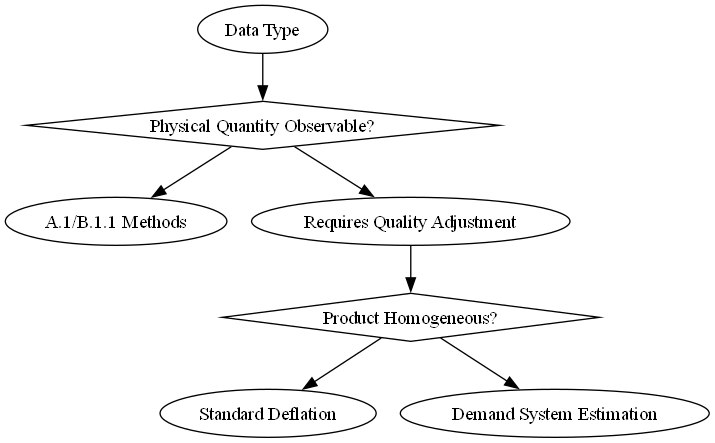
\includegraphics[width=\textwidth]{Figure/decision_tree.png}%
    }
    \end{column}
\end{columns}
\end{frame}


%Section 2
\section{Estimation Methods}
\subsection{Estimation Methods: Perfect Competition(A)}
\subsubsection{Factor Shares Approach(A.1)}
\begin{frame}{Factor Shares Approach(A.1)}
    \begin{block}{Theoretical Basis}
        \begin{columns}[t] % 使用 [t] 参数对齐列顶部
            % 第一列
            \begin{column}{0.48\textwidth} % 调整列宽
                Under cost minimization:
                \[
                \beta^H_{X} = \frac{1}{N_{t}}\sum_i \frac{P^{X^{H}}_{it} X^H_{it}}{TC_{it}}
                \]
            \end{column}
            % 第二列
            \begin{column}{0.48\textwidth} % 调整列宽
                At the firm level:
                \[
                \beta^H_{X} = \frac{P^{X^{H}}_{it} X^H_{it}}{TC_{it}}
                \]
            \end{column}
        \end{columns}
    \end{block}

    \begin{exampleblock}{Applicability Conditions}
        \begin{itemize}
            \item Perfect competition (A.1): Input's cost share equals its revenue share \(\frac{P^{X}X}{PQ}\).
            \item Constant returns to scale.
            \item No adjustment costs.
        \end{itemize}
    \end{exampleblock}

    \begin{alertblock}{Key Challenges}
        It requires accurate measurement of input cost shares.
    \end{alertblock}
\end{frame}

\subsubsection{Production Function Estimation(A.1/A.2)}
\begin{frame}{Production Function Estimation(A.1/A.2)}
\vspace{-0.3cm}
\begin{columns}[T]
    % Left Column
    \begin{column}{0.48\textwidth}
        \begin{block}{Core Specification}
            \vspace{-0.2cm}
            \begin{equation*}
                q_{it} = \underbrace{\beta_V x_{it}^V}_{\text{Variable}} + \underbrace{\beta_F x_{it}^F}_{\text{Fixed}} + \omega_{it} + \epsilon_{it}
            \end{equation*}
        \end{block}
        
        \begin{exampleblock}{Input Classification}
            \textbf{Variable Inputs} (\(x^V\))
            \begin{itemize}\setlength\itemsep{0.2em}
                \item Labor (\(L_{it}\))
                \item Materials (\(M_{it}\))
            \end{itemize}
            
            \textbf{Fixed Inputs} (\(x^F\))
            \begin{itemize}\setlength\itemsep{0.2em}
                \item Capital (\(K_{it}\))
            \end{itemize}
        \end{exampleblock}
    \end{column}
    
    % Right Column
    \begin{column}{0.48\textwidth}
        \begin{alertblock}{Key Parameters}
            \begin{itemize}
                \item \textbf{Output Elasticities}:
                \begin{equation*}
                    \beta_V = \frac{\partial \ln Q}{\partial \ln x^V}, \quad
                    \beta_F = \frac{\partial \ln Q}{\partial \ln x^F}
                \end{equation*}
                
                \item \textbf{TFP Decomposition}:
                \begin{equation*}
                    \omega_{it} = \ln\left(\frac{Q_{it}}{F(\cdot)}\right)
                \end{equation*}
                
                \item \textbf{Error Term}:
                \begin{equation*}
                    \epsilon_{it} \sim \mathcal{N}(0,\sigma_\epsilon^2)
                \end{equation*}
            \end{itemize}
        \end{alertblock}
    \end{column}
\end{columns}

\vspace{0.3cm}
\begin{center}
\footnotesize
\resizebox{\textwidth}{!}{ % 如果表格太宽,可以使用 resizebox 调整大小
\begin{tabular}{ll}
\toprule
\textbf{Symbol} & \textbf{Economic Meaning} \\
\midrule
\(\beta_V\) & Short-run production flexibility \\
\(\beta_F\) & Long-term capacity effect \\
\(\omega_{it}\) & Technical efficiency \\
\(\epsilon_{it}\) & Measurement noise \\
\bottomrule
\end{tabular}
}
\end{center}
\end{frame}


\begin{frame}{Production Function Estimation(A.1/A.2)}
    \begin{alertblock}{Key Challenges}
        \begin{itemize}
            \item Endogeneity bias (input choices correlated with productivity)
            \item Selection bias (exit of low-productivity firms)
        \end{itemize}
    \end{alertblock}


\textbf{Approaches to Address Challenges:}
    \begin{itemize}
        \item \textbf{Instrument Variables}
        \begin{itemize}
            \item Input price (usually not available to the econometrician)
            \item Demand-side shifters (affect the validity of the approach)
        \end{itemize}

        \item \textbf{Control Function Approach (Perfect Competition)}
        \begin{itemize}
            \item Olley-Pakes (1996): Investment policy function inversion
            \item Levinsohn-Petrin (2003): Intermediate inputs as proxy
            \item Ackerberg-Caves-Frazer (2015): Unified framework
            % \item Key equation: $\omega_{it} = g(\omega_{it-1}) + \xi_{it}$
        \end{itemize}

        \item \textbf{Dynamic Panel Approach (Arellano-Bond 1991)}
        \begin{itemize}
            \item AR(1) process: $\omega_{it} = \rho\omega_{it-1} + \xi_{it}$
            % \item GMM estimation with lagged instruments
            \item Capital coefficients are often low or even negative when estimated.
        \end{itemize}
    \end{itemize}
\end{frame}


\begin{frame}{Production Function Estimation: Control Function Approach }
    \begin{itemize}
        \item \textbf{Key Equations}:
    \end{itemize}
    \begin{align*}
        \text{Production function} &\quad q_{it} = \beta_V x_{it}^V + \beta_F x_{it}^F + \omega_{it} + \epsilon_{it} \\
        \text{Input demand} &\quad d_{it} = d_t(\omega_{it}, x_{it}^V, x_{it}^F) \\
        \text{Inverted Input demand} &\quad \omega_{it} = d_t^{-1}(d_{it}, x_{it}^V, x_{it}^F) \\
        \text{Productivity dynamics} &\quad \omega_{it} = g(\omega_{it-1}) + \xi_{it} \\
        \text{Capital accumulation equation} &\quad  K_{it} = (1-\delta)K_{it-1} + I_{it-1}
    \end{align*}
        \begin{itemize}
        \item \textbf{Key Assumptions}:
        \begin{itemize}
            \item Monotonicity condition: $d_{it}$ strictly monotonic in $\omega_{it}$. Unobserved productivity shock can be controlled and obviate the simultaneity problem.
            \item Productivity follows a first-order Markov process $\omega_{it} = g(\omega_{it-1}) + \xi_{it}$, which is a core time assumption and deals with selection bias.
        \end{itemize}
    \end{itemize}
\end{frame}


\begin{frame}{Production Function Estimation: Control Function Approach}
\textbf{Estimation Procedure: two-steps}
    \begin{itemize}
        \item \textbf{First Step: Output Prediction}
        \begin{itemize}
            \item Replace unobserved productivity $\omega_{it}$ with inverted input (investment or intermediate input) demand equation:
            \[
                \omega_{it} = d_t^{-1}(d_{it}, x_{it}^V, x_{it}^F)
            \]
            
            \item Construct predicted output equation:
            \[
                q_{it} = \phi_t(d_{it}, x_{it}^V, x_{it}^F) + \epsilon_{it}
            \]
            where $\phi_t(\cdot)$ captures predicted output:
            \[
                \phi_t(\cdot) = \beta_V x_{it}^V + \beta_F x_{it}^F + \omega_{it}
            \]
            
            \item Key purposes:
            \begin{itemize}
                \item Remove measurement error $\epsilon_{it}$
                \item Capture market-specific price variation through $\phi_t(\cdot)$
            \end{itemize}
        \end{itemize}
    \end{itemize}
\end{frame}


\begin{frame}{Production Function Estimation: Control Function Approach}
\begin{itemize}
    \item \textbf{Second Stage: Productivity Dynamics}
    \begin{itemize}
        \item Assume Markov productivity process:
        \[
            \omega_{it} = g(\omega_{it-1}) + \xi_{it}
        \]
        
        \item Compute productivity for parameter guess $\beta$:
        \[
            \omega_{it} = \hat{\phi}_{it} - \beta_V x_{it}^V - \beta_F x_{it}^F
        \]
        
        \item Form moment conditions:
        \[
            E\left[\xi_{it}(\beta) \begin{pmatrix} x_{it-s}^V \\ x_{it}^F \end{pmatrix}\right] = 0
        \]
        
        \item Critical timing assumptions:
        \begin{itemize}
            \item Variable inputs ($x^V$) react contemporaneously to productivity shock ($\xi_{it}$)
            \item Fixed inputs ($x^F$) follow dynamic accumulation:
            \[
                K_{it} = (1-\delta)K_{it-1} + I_{it-1}
            \]
        \end{itemize}
    \end{itemize}
\end{itemize}
\end{frame}


\begin{frame}{Production Function Estimation: Control Function Approach}
\textbf {Key Implementation Features}
\begin{itemize}
    \item \textbf{Input Differentiation}:
    \begin{itemize}
        \item Variable inputs ($x^V$): Intra-period adjustment (e.g., labor)
        \item Fixed inputs ($x^F$): Inter-temporal accumulation (e.g., capital)
    \end{itemize}
    
    \item \textbf{Identification Strategy}:
    \begin{itemize}
        \item Leverage differential timing of input adjustments
        \item Use lagged flexible inputs as instruments
        \item Exploit exogenous variation in fixed input accumulation
    \end{itemize}
    
    \item \textbf{Computational Procedure}:
    \begin{enumerate}
        \item Nonparametric estimation of $\phi_t(\cdot)$ (typically polynomial approximation)
        \item Nonlinear GMM estimation using moment conditions
        \item Bootstrap standard errors to account for generated regressors
    \end{enumerate}
\end{itemize}
\end{frame}




\subsection{Estimation Methods: Imperfect Competition(B)}
\subsubsection{A serious approaches: Imperfect Competition (B.1/B.2)}
% 第一页幻灯片:Core Challenges
\begin{frame}{Production Function Estimation: Imperfect Competition (B)}
\textbf{Core Challenges}
\begin{itemize}
    \item \textbf{Output-Input Comparability}:
    \begin{itemize}
        \item Differentiated products create non-comparable physical units(B.2)
        \item Revenue/expenditure data introduce price heterogeneity (Price Deflation Approaches)
        \item Example: Luxury vs economy cars cannot be directly compared
    \end{itemize}
    
    \item \textbf{Price Heterogeneity Bias}:
    \begin{itemize}
        \item Unobserved price variations contaminate productivity measures (Demand System Integration)
        \item High prices may reflect quality/market power rather than efficiency (Quality-Adjusted)
        \item TFPR (Revenue-based TFP) vs TFPQ (Quantity-based TFP) distinction (Demand System Integration)
    \end{itemize}
\end{itemize}

\end{frame}


% 第二页幻灯片:Methodological Framework (Control Function Modifications)
% \begin{frame}{Control Function Approach Imperfect Competition)(B.1)}
% \begin{itemize}
%     \item Extended input demand equation:
%     \[
%     d_{it} = d_t(\omega_{it}, x^V_{it}, x^F_{it}, \mathbf{z}_{it})
%     \]
%     Where $\mathbf{z}_{it}$ includes:
%     \begin{itemize}
%         \item Demand shifters (market shares, product characteristics)
%         \item Input price variation
%         \item Strategic variables (competitors' productivity)
%     \end{itemize}
    
%     \item Required inversion condition:
%     \[
%     \omega_{it} = d^{-1}_t(d_{it}, x^V_{it}, x^F_{it}, \mathbf{z}_{it})
%     \]
% \end{itemize}
% \end{frame}

% 第二页幻灯片:Methodological Solutions (Price Deflation)
\begin{frame}{Price Deflation Approaches}

\textbf {Converts observed revenue to output data using additional price data}
\begin{itemize}
    \item \textbf{Industry-level Deflation}:
    \[
    Q_{it} = \frac{R_{it}}{P_t} \quad \text{(Standard practice but insufficient)}
    \]
    \begin{itemize}
        \item Removes common price trends from revenue data
        \item Fails to address cross-producer price differences
    \end{itemize}
    
    \item \textbf{Producer-level Deflation}:
    \[
    Q_{it} = \frac{R_{it}}{P_{it}} \quad \text{(Requires product-specific price data)}
    \]
    \begin{itemize}
        \item Enables quality-adjusted quantity comparison
        \item Implementation challenges in multi-product firms
    \end{itemize}
\end{itemize}
\end{frame}

% 第三页幻灯片:Methodological Solutions (Demand System Integration)
\begin{frame}{Demand System Integration}
\begin{itemize}
\item \textbf{Motivation}: 
    \begin{itemize}
        \item Traditional approaches \alert{ignore price measurement error}, leading to:
        \begin{itemize}
            \item Downward bias in returns-to-scale estimates
            \item Confounded demand shocks and productivity effects
        \end{itemize}
    \end{itemize}
    \item \textbf{Nested CES demand system (De Loecker, 2011)}:
    \[
    Q_{it} = Q_t\left(\frac{P_{it}}{P_t}\right)^\psi \exp(\nu_{it})
    \]
    \begin{itemize}
        \item $\psi$: Demand elasticity
        \item $\nu_{it}$: Idiosyncratic demand shock
    \end{itemize}
    
    \item \textbf{Revenue production function with price correction:}:
    \[
    r_{it} - p_t = \alpha_{V}x^{V}_{it} + \frac{1}{|\psi|}q_t + \tilde{\omega}_{it} + \tilde{\epsilon}_{it}
    \]
   \item Joint identification of: Production elasticity ($\alpha_V=(\frac{\psi+1}{\psi})\beta_{V}$)
\end{itemize}
\end{frame}

% 第四页幻灯片:Methodological Solutions (Quality-Adjusted Production Functions)
\begin{frame}{Quality-Adjusted Production Functions (Product Differentiation)}
\begin{itemize}
    \item \textbf{Assumption}: 
    \begin{itemize}
        \item products where higher-quality version (whose producers can sell for higher prices) require higher-quality inputs (whose producers must pay more to obtain) 
    \end{itemize}
    \item \textbf{Vertical Differentiation Model}:
    \[
    Q(\nu) = F(X^V(\nu))\Omega
    \]
    \begin{itemize}
        \item $\nu$: Product quality (inferred from prices)
        \item Price-quality mapping: $\nu = v(p_{it})$
    \end{itemize}
    
    \item \textbf{Empirical Implementation}:
    \[
    q_{it} = \beta_V x_{it}^V + \omega_{it} + v(p_{it}) + \epsilon_{it}
    \]
   \item Identification via: uses lagged prices as instruments for quality shocks and price quality mapping $\nu = v(p_{it})$
\end{itemize}
\end{frame}


% % 第五页幻灯片:Empirical Implications
% \begin{frame}{Empirical Implications}
% \subsection{Empirical Implications}
% \begin{itemize}
%     \item \textbf{Scale Elasticity Underestimation}:
%     \begin{itemize}
%         \item Ignoring price heterogeneity underestimates returns to scale by 15-20\% (De Loecker, 2011a)
%     \end{itemize}
    
%     \item \textbf{Policy Evaluation Bias}:
%     \begin{itemize}
%         \item Trade reforms' productivity effects overestimated without demand controls (Roberts et al., 2017)
%     \end{itemize}
    
%     \item \textbf{Input-Output Price Correlation}:
%     \begin{itemize}
%         \item High-quality producers face both output premium and input cost premium
%         \item Requires simultaneous price adjustment
%     \end{itemize}
% \end{itemize}
% \end{frame}

% % 第六页幻灯片:Frontier Methods
% \begin{frame}{Frontier Methods}
% \subsection{Frontier Methods}
% \begin{itemize}
%     \item \textbf{Pass-Through Approach}:
%     \[
%     \tilde{\omega}_{it} = \omega_{it} + p_{it} - \beta_V p_{it}^V
%     \]
%     Exploits systematic input-output price relationships
    
%     \item \textbf{Nonparametric Identification}:
%     \begin{itemize}
%         \item Gandhi et al. (2020): Combines factor shares with Markov processes
%         \item Requires high-frequency price data
%     \end{itemize}
    
%     \item \textbf{Oligopoly Competition Models}:
%     \begin{itemize}
%         \item Strategic interactions affect input demand equations
%         \item Requires game-theoretic extensions to control functions
%     \end{itemize}
% \end{itemize}
% \end{frame}



\begin{frame}{Method Comparison}
\begin{table}[h]
\centering
\caption{2 Method Comparison}
\resizebox{\textwidth}{!}{ % 调整表格大小以适应幻灯片
\begin{tabular}{lcc}
\toprule
Approach & Data Requirements & Key Limitation \\
\midrule
Industry Deflation & Aggregate price indices & Ignores firm-level price variation \\
Demand System & Product-level quantities & Requires demand shifters \\
Quality Adjustment & Firm-specific prices & Assumes vertical differentiation \\
\bottomrule
\end{tabular}
}
\end{table}
\end{frame}


\subsection{Estimation Methods: Multi-product Production (A.2/B.2)}
\begin{frame}{Estimation Methods: Multi-product Production (A.2/B.2)}
\textbf{Basic Framework}:
Given a multi-product producer, we start with the product-level production function:
\begin{equation*}
Q_j = \left(X^V_j\right)^{\beta_V} \left(X^F_j\right)^{\beta_F}\Omega
\end{equation*}
where:
\begin{itemize}
    \item \( Q_j \): Output of product \( j \)
    \item \( X^V_j, X^F_j \): Variable and fixed inputs allocated to product \( j \)
    \item \( \beta_V, \beta_F \): Output elasticities of inputs
\end{itemize}
Under two critical assumptions:
\begin{enumerate}
    \item \textbf{Common Productivity}: Productivity \( \omega_{it} \) is identical across all products within a firm
    \item \textbf{Neutral Input Allocation}: Inputs allocated proportionally to products via shares \( a_j \):
    \[
    X^H_j = a_j X^H \quad \forall H \in \{V,F\}
    \]
\end{enumerate}
\end{frame}


\begin{frame}{Aggregation Procedure  }
\begin{enumerate}
    \item \textbf{Data Inputs}:
    \begin{itemize}
        \item Product-level outputs ($Q_j$): Typically revenue data
        \item Firm-level inputs ($X^V, X^F$): No product breakdown
    \end{itemize}
    
    \item \textbf{Allocation Rules}:
    \[
    a_j = \begin{cases}
        \frac{1}{J} & \text{(Equal share, number of products)} \\
        \frac{Q_{j}}{Q} & \text{(Output share, Revenue/Physical output)}
    \end{cases}
    \]
    
    \item \textbf{Aggregation Formula} (CRS):
    \[
    Q = \sum_j Q_j =\sum_{j}\alpha_{j}^{\beta_{V}+\beta_{F}} (X^V)^{\beta_{V}} (X^F)^{\beta_{F}}\Omega \quad \text{if } \beta_V + \beta_F = 1
    \]
 \textbf{Non-CRS Case}: 
        Requires additional terms (e.g., log number of products \( \ln J \)) and addresses endogeneity of product count \( J \)
\end{enumerate}
\end{frame}

\subsubsection{Estimate Transformation Function (A.2)}
\begin{frame}{Estimate Transformation Function (A.2)}
\textbf{Study Reference:} Dhyne et al. (2014) 
 \begin{itemize}
        \item Focus: Production in Belgian bakeries producing bread and pastries.
        \item Assumption: Both products (bread and pastries) are homogeneous.
    \end{itemize}
\begin{align*}
    q_1 &= \gamma_1 q_2 + \beta_V^1 x^V + \beta_F^1 x^F + \omega_1  \\
    q_2 &= \gamma_2 q_1 + \beta_V^2 x^V + \beta_F^2 x^F + \omega_2 
\end{align*}

\vspace{0.1cm}
\begin{table}[h]
\centering
\resizebox{\textwidth}{!}{ % 调整表格大小以适应幻灯片宽度
\begin{tabular}{ll}
\toprule
\textbf{Parameter} & \textbf{Meaning} \\
\midrule
$\gamma_j$ & Inter-product interaction effect: \\
           & $\gamma_j < 0$: Resource competition (e.g., $\gamma_1 < 0$ implies 1 output decreases with 2 production) \\
           & $\gamma_j > 0$: Synergy effect (e.g., $\gamma_2 > 0$ suggests 2 efficiency gains from 1 production) \\
$\beta_V^j$ & Variable input elasticity for product $j$ \\
$\beta_F^j$ & Fixed input elasticity for product $j$ \\
$\omega_j$ & Product-specific productivity shock \\
\bottomrule
\end{tabular}
}
\end{table}
\end{frame}



\begin{frame}{Fundamental Issues}
\begin{itemize}
    \item \textbf{Multiple Unobservables}:
    \begin{itemize}
        \item $J$ productivity terms: $\omega_{i1t}, \omega_{i2t}, \dots, \omega_{iJt}$
        \item Traditional single-product models only handle $\omega_{it}$
        \item Total parameters must be estimated: $J\text{ (products)} + 2J\text{ (input elasticities)} = 3J$ \\
              \textit{(Example: 6 parameters when $J=2$)}
    \end{itemize}
    
    \item \textbf{Endogeneity Problems}:
    \begin{itemize}
        \item Simultaneity: $q_{-j,t}$ as endogenous regressor
        \item High-dimensional instrumentation: Requires $(J-1)$ valid instruments
    \end{itemize}
\end{itemize}

\begin{alertblock}{Key Complexity}
Model complexity grows exponentially with product count $J$
\end{alertblock}
\end{frame}

\begin{frame}{Control Function Extension}
    \textbf{Data Description:}
    \begin{itemize}
        \item Quantities produced for each product are reported.
        \item Total input use is reported, distinguishing between:
        \begin{itemize}
            \item Variable factors of production.
            \item Fixed factors of production.
        \end{itemize}
    \end{itemize}

\textbf{Dhyne et al. (2014) Solution}:
\begin{itemize}
    \item Combines OP (investment) and LP (materials) proxies:
    \[
    \begin{pmatrix}
    \omega_{i1t} \\
    \omega_{i2t}
    \end{pmatrix} = h_t(k_{it}, m_{it}, i_{it})
    \]
    \item Requires bijective mapping $h_t(\cdot)$
    \item Limited to $J=2$ case (bread \& pastries)
\end{itemize}
This further highlights the additional restrictions required of the control function approach in this scenario.

\end{frame}


\subsubsection{Product Differentiation (B.2)}
% Page 1: Core Challenges
\begin{frame}{Product Differentiation (B.2)}
\begin{itemize}
    \item \textbf{Product Differentiation Bias}:
    \begin{itemize}
        \item Traditional deflation methods fail under quality heterogeneity
        \item Unobserved input price variations confound elasticity estimates
        \item Example: Premium flour inputs correlate with bread quality
    \end{itemize}
    
    \item \textbf{Identification Complexity}:
    \begin{itemize}
        \item Requires separating demand shocks from productivity effects
        \item Needs product-level price/quality adjustments
    \end{itemize}
\end{itemize}
\end{frame}

% Page 2: Methodological Framework
\begin{frame}{Methodological Framework}
\begin{itemize}
    \item \textbf{Key Assumptions}:
    \begin{enumerate}
        \item Product-specific production functions:
        \[
        Q_1 = F_1(X_1)\Omega_{1},\ Q_2 = F_2(X_2)\Omega_{2}
        \]
        \item Firm-level productivity ($\omega$), no physical synergies
            \[
    q_1 = \beta_{V_1} x_{1}^V + \beta_{F_{1}} x_{1}^F + \omega 
    \]
    \[
    q_2 = \beta_{V_{2}} x_{2}^V + \beta_{F_{2}} x_{2}^F + \omega 
    \]
    \end{enumerate}
\end{itemize}

\begin{alertblock}{Scope Restriction}
Excludes equipment sharing efficiencies but allows:
\begin{itemize}
    \item Shared fixed costs:

    \item Bulk purchase discounts:
    \[
    C(Q_1, Q_2) \leq C(Q_1) + C(Q_2)
    \]
\end{itemize}
\end{alertblock}
\end{frame}

% Page 3: Estimation Procedure
\begin{frame}{Estimation Procedure}
\begin{enumerate}
    \item \textbf{Input Allocation}:
    Define allocation shares (\(\rho_j\)) based on expenditure:
    \[
    \exp(\rho_j) = \frac{P_{j}^{H} X_j^H}{\sum_j P_{j}^{H} X_j^H}, \quad H \in \{V, F\}
    \]
    This ensures full input allocation:
    \[
    \sum_j \exp(\rho_j) = 1
    \]

    \item \textbf{System of Equations}:
    Solve the following system of equations:
    \[
    \begin{cases}
    q_1 - \beta_{V_1} x^V - \beta_{F_1} x^F = \rho_1 + \omega \\
    q_2 - \beta_{V_1} x^V - \beta_{F_2} x^F = \rho_2 + \omega
    \end{cases}
    \]
    Unknowns: \(\rho_1, \rho_2, \omega\).

\end{enumerate}
\end{frame}


% Page 1: Simplified CRS Case
\begin{frame}{Simplified CRS Illustration}
\begin{itemize}
    \item \textbf{Common Technology Assumption}:
    \[
    \beta_V^1 = \beta_V^2,\quad \beta_F^1 = \beta_F^2
    \]
    
    \item \textbf{Input Allocation Rule}:
    \[
    \exp(\rho_j) = \frac{Q_j}{\sum_j Q_j}
    \]
    
    \item \textbf{Productivity Metric}:
    \[
    \Omega = \frac{\sum_j Q_j}{X},\quad \ln X = \beta_V x^V + \beta_F x^F
    \]
\end{itemize}
\end{frame}

% Page 2: Generalized Framework
\begin{frame}{Generalized Framework Features}
\begin{itemize}
    \item \textbf{Extended Capabilities}:
    \begin{itemize}
        \item Product-specific technologies (\(\beta_V^j \neq \beta_V^k\))
        \item Variable returns to scale (\(\beta_V^j + \beta_F^j \neq 1\))
        \item Quality-adjusted differentiation (\(Q_j = \nu_j F_j(X_j)\))
    \end{itemize}
    
    \item \textbf{Key Requirements}:
    \begin{enumerate}
        \item Single-product producer samples for baseline estimation
        \item Cost traceability to products
        \item Product-specific (not factor-specific) allocation
    \end{enumerate}
\end{itemize}

\begin{alertblock}{Critical Insight}
Quality differentiation requires price-quality mapping:
\[
\nu_j = v(p_j)
\]
\end{alertblock}
\end{frame}



\section{Discussion}
\subsection{Cost versus Production Functions}
\begin{frame}{Deriving the Cost Function}
Starting from the production function and solving a static cost minimization problem (equating the marginal rate of technical substitution to input price ratios), we derive the log-linear cost function:
\[
\ln C_{it} = c_0 + \frac{1}{\beta_V + \beta_F} q_{it} + \frac{\beta_V}{\beta_V + \beta_F} p^V_{it} + \frac{\beta_F}{\beta_V + \beta_F} p^F_{it} + \frac{1}{\beta_V + \beta_F} \omega_{it} + \epsilon_{it}^* 
\]
where:
\begin{itemize}
    \item \(C_{it}\): Total cost of firm \(i\) at time \(t\)
    \item \(q_{it}\): Output quantity
    \item \(p^V_{it}, p^F_{it}\): Prices of variable and fixed inputs
    \item \(\omega_{it}\): Unobserved productivity shocks
    \item \(\epsilon_{it}^*\): Measurement error
\end{itemize}
\end{frame}

\begin{frame}{Methodological Comparison}
    
\begin{itemize} 
    \item \textbf{Data Requirements}:
    \begin{itemize}
        \item Observability of factor prices (\(p^V_{it}, p^F_{it}\))
        \item Accurate measurement of economic costs (\(C_{it}\))
    \end{itemize}
\end{itemize}

\begin{table}[h]
\centering
\caption{3 Cost Function vs. Production Function Approaches}
\begin{tabular}{p{0.45\textwidth}p{0.45\textwidth}}
\toprule
\textbf{Cost Function Approach} & \textbf{Production Function Approach} \\
\midrule
Requires cost data and input prices & Requires input quantities and output data \\
Easily handles scale/scope economies & Requires explicit modeling of multi-product production \\
Assumes cost minimization & Assumes exogenous productivity \\
Sensitive to input price measurement & Sensitive to input quantity measurement \\
\bottomrule
\end{tabular}
\end{table}
\end{frame}

\subsection{Measurement and Specification Errors}
% Page 1: Measurement Errors
\begin{frame}{Capital Measurement}
\begin{itemize}
    \item \textbf{Sources}:
    \begin{itemize}
        \item Asset heterogeneity (varying equipment lifespans)
        \item Depreciation rate misspecification
        \item Unadjusted capital price fluctuations
    \end{itemize}
    
    \item \textbf{Impact}:
    \begin{itemize}
        \item Biased capital elasticity (\(\beta_F\))
        \item Distorted productivity estimates
    \end{itemize}
    
    \item \textbf{Solutions}:
    \begin{itemize}
        \item Instrumental Variables (lagged investment)
        \item Nonparametric methods (Kim et al., 2016)
    \end{itemize}
\end{itemize}
\end{frame}

% Page 2: Specification Errors
\begin{frame}{Specification Errors}
\begin{itemize}
    \item \textbf{Problem}: Omitting drivers (e.g., R\&D \(A_{it}\)):
    \[
    \omega_{it} = g(\omega_{it-1}) + \xi_{it} \quad (\text{Missing } A_{it-s})
    \]
    
    \item \textbf{Solution}: Enhanced dynamic equation
    \[
    \omega_{it} = g(\omega_{it-1}, A_{it-s}) + \xi_{it}
    \]
\end{itemize}

\begin{itemize}
    \item \textbf{Cobb-Douglas Limitation}: Fixed substitution elasticity (\(\sigma=1\))
    \item \textbf{Alternatives}:
    \begin{itemize}
        \item Translog: Flexible elasticities (De Loecker \& Warzynski, 2012)
        \item CES: Free substitution parameter
        \item Nonparametric: Gandhi et al. (2020)
    \end{itemize}
\end{itemize}
\end{frame}

% Page 3: Empirical Implications
\begin{frame}{Empirical Implications \& Solutions}
\begin{table}[ht]
\centering
\caption{4 Error Types \& Remedies}
\begin{tabular}{p{3cm}p{4cm}p{4cm}}
\toprule
\textbf{Error Type} & \textbf{Impact} & \textbf{Solution} \\
\midrule
Capital Measurement & \(\beta_F\) attenuation & IVs, Nonparametric CF \\
Output Measurement & \(\omega_{it}\) volatility & Two-stage CF, GMM \\
Process Misspecification & R\&D effect bias & Enriched dynamics \\
Technological Heterogeneity & Diffusion misjudgment & Multi-technology models \\
Functional Form & Scale/elasticity bias & Translog/CES \\
\bottomrule
\end{tabular}
\end{table}
\end{frame}



\begin{frame}{Decision Tree Visualization}
\hypertarget{imagepage}{} 
\centering
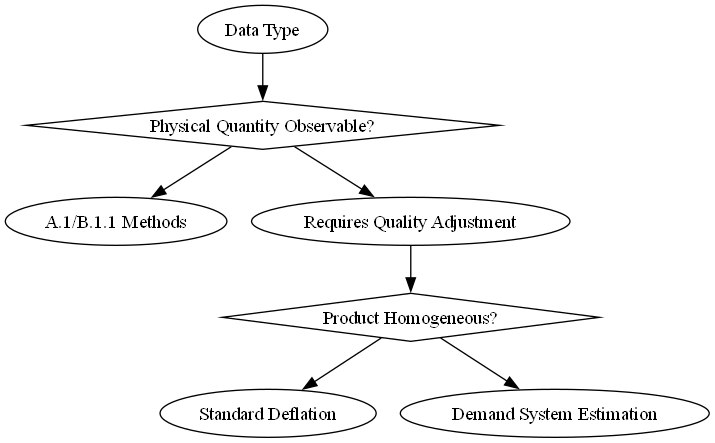
\includegraphics[width=0.8\textwidth]{Figure/decision_tree.png}

\vspace{1em}
\hyperlink{mainpage}{\beamerbutton{Back to Main Page}}
\end{frame}


\begin{frame}[plain]
    \centering
    \vspace{2cm}
    {\Huge \textbf{Thank You!}}
\end{frame}


\end{document}


